\documentclass[twoside]{book}

% Packages required by doxygen
\usepackage{fixltx2e}
\usepackage{calc}
\usepackage{doxygen}
\usepackage[export]{adjustbox} % also loads graphicx
\usepackage{graphicx}
\usepackage[utf8]{inputenc}
\usepackage{makeidx}
\usepackage{multicol}
\usepackage{multirow}
\PassOptionsToPackage{warn}{textcomp}
\usepackage{textcomp}
\usepackage[nointegrals]{wasysym}
\usepackage[table]{xcolor}

% Font selection
\usepackage[T1]{fontenc}
\usepackage[scaled=.90]{helvet}
\usepackage{courier}
\usepackage{amssymb}
\usepackage{sectsty}
\renewcommand{\familydefault}{\sfdefault}
\allsectionsfont{%
  \fontseries{bc}\selectfont%
  \color{darkgray}%
}
\renewcommand{\DoxyLabelFont}{%
  \fontseries{bc}\selectfont%
  \color{darkgray}%
}
\newcommand{\+}{\discretionary{\mbox{\scriptsize$\hookleftarrow$}}{}{}}

% Page & text layout
\usepackage{geometry}
\geometry{%
  a4paper,%
  top=2.5cm,%
  bottom=2.5cm,%
  left=2.5cm,%
  right=2.5cm%
}
\tolerance=750
\hfuzz=15pt
\hbadness=750
\setlength{\emergencystretch}{15pt}
\setlength{\parindent}{0cm}
\setlength{\parskip}{3ex plus 2ex minus 2ex}
\makeatletter
\renewcommand{\paragraph}{%
  \@startsection{paragraph}{4}{0ex}{-1.0ex}{1.0ex}{%
    \normalfont\normalsize\bfseries\SS@parafont%
  }%
}
\renewcommand{\subparagraph}{%
  \@startsection{subparagraph}{5}{0ex}{-1.0ex}{1.0ex}{%
    \normalfont\normalsize\bfseries\SS@subparafont%
  }%
}
\makeatother

% Headers & footers
\usepackage{fancyhdr}
\pagestyle{fancyplain}
\fancyhead[LE]{\fancyplain{}{\bfseries\thepage}}
\fancyhead[CE]{\fancyplain{}{}}
\fancyhead[RE]{\fancyplain{}{\bfseries\leftmark}}
\fancyhead[LO]{\fancyplain{}{\bfseries\rightmark}}
\fancyhead[CO]{\fancyplain{}{}}
\fancyhead[RO]{\fancyplain{}{\bfseries\thepage}}
\fancyfoot[LE]{\fancyplain{}{}}
\fancyfoot[CE]{\fancyplain{}{}}
\fancyfoot[RE]{\fancyplain{}{\bfseries\scriptsize Generated by Doxygen }}
\fancyfoot[LO]{\fancyplain{}{\bfseries\scriptsize Generated by Doxygen }}
\fancyfoot[CO]{\fancyplain{}{}}
\fancyfoot[RO]{\fancyplain{}{}}
\renewcommand{\footrulewidth}{0.4pt}
\renewcommand{\chaptermark}[1]{%
  \markboth{#1}{}%
}
\renewcommand{\sectionmark}[1]{%
  \markright{\thesection\ #1}%
}

% Indices & bibliography
\usepackage{natbib}
\usepackage[titles]{tocloft}
\setcounter{tocdepth}{3}
\setcounter{secnumdepth}{5}
\makeindex

% Hyperlinks (required, but should be loaded last)
\usepackage{ifpdf}
\ifpdf
  \usepackage[pdftex,pagebackref=true]{hyperref}
\else
  \usepackage[ps2pdf,pagebackref=true]{hyperref}
\fi
\hypersetup{%
  colorlinks=true,%
  linkcolor=blue,%
  citecolor=blue,%
  unicode%
}

% Custom commands
\newcommand{\clearemptydoublepage}{%
  \newpage{\pagestyle{empty}\cleardoublepage}%
}

\usepackage{caption}
\captionsetup{labelsep=space,justification=centering,font={bf},singlelinecheck=off,skip=4pt,position=top}

%===== C O N T E N T S =====

\begin{document}

% Titlepage & ToC
\hypersetup{pageanchor=false,
             bookmarksnumbered=true,
             pdfencoding=unicode
            }
\pagenumbering{alph}
\begin{titlepage}
\vspace*{7cm}
\begin{center}%
{\Large Programmieren-\/\+Enigma \\[1ex]\large 1.\+0 }\\
\vspace*{1cm}
{\large Generated by Doxygen 1.8.13}\\
\end{center}
\end{titlepage}
\clearemptydoublepage
\pagenumbering{roman}
\tableofcontents
\clearemptydoublepage
\pagenumbering{arabic}
\hypersetup{pageanchor=true}

%--- Begin generated contents ---
\chapter{Hierarchical Index}
\section{Class Hierarchy}
This inheritance list is sorted roughly, but not completely, alphabetically\+:\begin{DoxyCompactList}
\item \contentsline{section}{de.\+Enigma.\+Algorithm.\+Algorithm}{\pageref{classde_1_1_enigma_1_1_algorithm_1_1_algorithm}}{}
\begin{DoxyCompactList}
\item \contentsline{section}{de.\+Enigma.\+Algorithm.\+Decryptor}{\pageref{classde_1_1_enigma_1_1_algorithm_1_1_decryptor}}{}
\item \contentsline{section}{de.\+Enigma.\+Algorithm.\+Encryptor}{\pageref{classde_1_1_enigma_1_1_algorithm_1_1_encryptor}}{}
\end{DoxyCompactList}
\item \contentsline{section}{de.\+Enigma.\+Algorithm.\+Algorithm\+Controller}{\pageref{classde_1_1_enigma_1_1_algorithm_1_1_algorithm_controller}}{}
\item \contentsline{section}{de.\+Enigma.\+Util.\+Enums.\+E\+Alphabet}{\pageref{enumde_1_1_enigma_1_1_util_1_1_enums_1_1_e_alphabet}}{}
\item \contentsline{section}{de.\+Enigma.\+Util.\+Enums.\+E\+Mill}{\pageref{enumde_1_1_enigma_1_1_util_1_1_enums_1_1_e_mill}}{}
\item \contentsline{section}{de.\+Enigma.\+Util.\+Enums.\+E\+Mill\+Alphabet}{\pageref{enumde_1_1_enigma_1_1_util_1_1_enums_1_1_e_mill_alphabet}}{}
\item \contentsline{section}{de.\+Enigma.\+Util.\+Enums.\+E\+Mode}{\pageref{enumde_1_1_enigma_1_1_util_1_1_enums_1_1_e_mode}}{}
\item \contentsline{section}{de.\+Enigma.\+Algorithm.\+Enigma\+Config}{\pageref{classde_1_1_enigma_1_1_algorithm_1_1_enigma_config}}{}
\item \contentsline{section}{de.\+Enigma.\+Util.\+Enums}{\pageref{classde_1_1_enigma_1_1_util_1_1_enums}}{}
\item \contentsline{section}{de.\+Enigma.\+Util.\+File\+Handler}{\pageref{classde_1_1_enigma_1_1_util_1_1_file_handler}}{}
\item \contentsline{section}{de.\+Enigma.\+U\+I.\+G\+UI}{\pageref{classde_1_1_enigma_1_1_u_i_1_1_g_u_i}}{}
\item \contentsline{section}{de.\+Enigma.\+Core.\+Log}{\pageref{classde_1_1_enigma_1_1_core_1_1_log}}{}
\item \contentsline{section}{de.\+Enigma.\+Core.\+Main}{\pageref{classde_1_1_enigma_1_1_core_1_1_main}}{}
\item \contentsline{section}{de.\+Enigma.\+Algorithm.\+Mill}{\pageref{classde_1_1_enigma_1_1_algorithm_1_1_mill}}{}
\item \contentsline{section}{de.\+Enigma.\+Util.\+Util}{\pageref{classde_1_1_enigma_1_1_util_1_1_util}}{}
\end{DoxyCompactList}

\chapter{Class Index}
\section{Class List}
Here are the classes, structs, unions and interfaces with brief descriptions\+:\begin{DoxyCompactList}
\item\contentsline{section}{\hyperlink{classde_1_1_enigma_1_1_algorithm_1_1_algorithm}{de.\+Enigma.\+Algorithm.\+Algorithm} }{\pageref{classde_1_1_enigma_1_1_algorithm_1_1_algorithm}}{}
\item\contentsline{section}{\hyperlink{classde_1_1_enigma_1_1_algorithm_1_1_algorithm_controller}{de.\+Enigma.\+Algorithm.\+Algorithm\+Controller} }{\pageref{classde_1_1_enigma_1_1_algorithm_1_1_algorithm_controller}}{}
\item\contentsline{section}{\hyperlink{classde_1_1_enigma_1_1_algorithm_1_1_decryptor}{de.\+Enigma.\+Algorithm.\+Decryptor} }{\pageref{classde_1_1_enigma_1_1_algorithm_1_1_decryptor}}{}
\item\contentsline{section}{\hyperlink{enumde_1_1_enigma_1_1_util_1_1_enums_1_1_e_alphabet}{de.\+Enigma.\+Util.\+Enums.\+E\+Alphabet} \\*) Ein Enum, welches das \char`\"{}normale\char`\"{} Alphabet enthält }{\pageref{enumde_1_1_enigma_1_1_util_1_1_enums_1_1_e_alphabet}}{}
\item\contentsline{section}{\hyperlink{enumde_1_1_enigma_1_1_util_1_1_enums_1_1_e_mill}{de.\+Enigma.\+Util.\+Enums.\+E\+Mill} \\*) Dieses Enum wird dazu verwendet, um die Instanzen der Walzen der Enigma anzusprechen, bzw. zwischen ihnen zu differenzieren }{\pageref{enumde_1_1_enigma_1_1_util_1_1_enums_1_1_e_mill}}{}
\item\contentsline{section}{\hyperlink{enumde_1_1_enigma_1_1_util_1_1_enums_1_1_e_mill_alphabet}{de.\+Enigma.\+Util.\+Enums.\+E\+Mill\+Alphabet} \\*) Dieses Enum enthält hauptsächlich die Alphabete für die Walzen 1-\/5 und die Umkehrwalzen A,B,C, welche in der Enigma I verbaut wurden }{\pageref{enumde_1_1_enigma_1_1_util_1_1_enums_1_1_e_mill_alphabet}}{}
\item\contentsline{section}{\hyperlink{enumde_1_1_enigma_1_1_util_1_1_enums_1_1_e_mode}{de.\+Enigma.\+Util.\+Enums.\+E\+Mode} \\*) Benutzt für die Übergabe des gewählten Modus der Enigma }{\pageref{enumde_1_1_enigma_1_1_util_1_1_enums_1_1_e_mode}}{}
\item\contentsline{section}{\hyperlink{classde_1_1_enigma_1_1_algorithm_1_1_encryptor}{de.\+Enigma.\+Algorithm.\+Encryptor} }{\pageref{classde_1_1_enigma_1_1_algorithm_1_1_encryptor}}{}
\item\contentsline{section}{\hyperlink{classde_1_1_enigma_1_1_algorithm_1_1_enigma_config}{de.\+Enigma.\+Algorithm.\+Enigma\+Config} \\*) Klasse, welche essenziell für die Verschlüsselung ist ( }{\pageref{classde_1_1_enigma_1_1_algorithm_1_1_enigma_config}}{}
\item\contentsline{section}{\hyperlink{classde_1_1_enigma_1_1_util_1_1_enums}{de.\+Enigma.\+Util.\+Enums} \\*) Klasse, welche verschiedene \hyperlink{classde_1_1_enigma_1_1_util_1_1_enums}{Enums} enthält, welche verschiedene Aufgaben erfüllen }{\pageref{classde_1_1_enigma_1_1_util_1_1_enums}}{}
\item\contentsline{section}{\hyperlink{classde_1_1_enigma_1_1_util_1_1_file_handler}{de.\+Enigma.\+Util.\+File\+Handler} }{\pageref{classde_1_1_enigma_1_1_util_1_1_file_handler}}{}
\item\contentsline{section}{\hyperlink{classde_1_1_enigma_1_1_u_i_1_1_g_u_i}{de.\+Enigma.\+U\+I.\+G\+UI} }{\pageref{classde_1_1_enigma_1_1_u_i_1_1_g_u_i}}{}
\item\contentsline{section}{\hyperlink{classde_1_1_enigma_1_1_core_1_1_log}{de.\+Enigma.\+Core.\+Log} \\*) Logger Klasse die eine in C++ geschriebene .dll einbindet, um die Logs zu schreiben ( }{\pageref{classde_1_1_enigma_1_1_core_1_1_log}}{}
\item\contentsline{section}{\hyperlink{classde_1_1_enigma_1_1_core_1_1_main}{de.\+Enigma.\+Core.\+Main} }{\pageref{classde_1_1_enigma_1_1_core_1_1_main}}{}
\item\contentsline{section}{\hyperlink{classde_1_1_enigma_1_1_algorithm_1_1_mill}{de.\+Enigma.\+Algorithm.\+Mill} \\*) Walzen Klasse, welche eine Walze der Enigma darstellt ( }{\pageref{classde_1_1_enigma_1_1_algorithm_1_1_mill}}{}
\item\contentsline{section}{\hyperlink{classde_1_1_enigma_1_1_util_1_1_util}{de.\+Enigma.\+Util.\+Util} }{\pageref{classde_1_1_enigma_1_1_util_1_1_util}}{}
\end{DoxyCompactList}

\chapter{Class Documentation}
\hypertarget{classde_1_1_enigma_1_1_algorithm_1_1_algorithm}{}\section{de.\+Enigma.\+Algorithm.\+Algorithm Class Reference}
\label{classde_1_1_enigma_1_1_algorithm_1_1_algorithm}\index{de.\+Enigma.\+Algorithm.\+Algorithm@{de.\+Enigma.\+Algorithm.\+Algorithm}}
Inheritance diagram for de.\+Enigma.\+Algorithm.\+Algorithm\+:\begin{figure}[H]
\begin{center}
\leavevmode
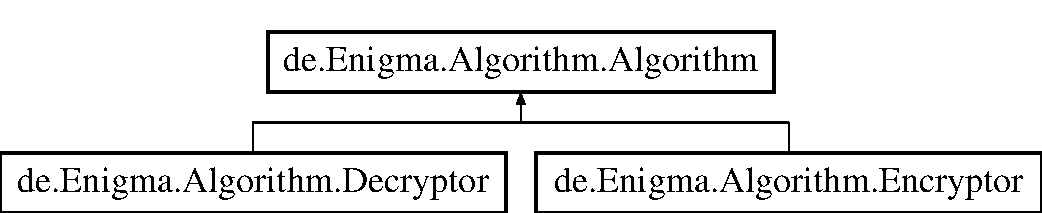
\includegraphics[height=2.000000cm]{classde_1_1_enigma_1_1_algorithm_1_1_algorithm}
\end{center}
\end{figure}
\subsection*{Protected Member Functions}
\begin{DoxyCompactItemize}
\item 
\mbox{\Hypertarget{classde_1_1_enigma_1_1_algorithm_1_1_algorithm_abf73078c3a282239deb76369616eec3d}\label{classde_1_1_enigma_1_1_algorithm_1_1_algorithm_abf73078c3a282239deb76369616eec3d}} 
char {\bfseries encrypt} (char letter)
\item 
\mbox{\Hypertarget{classde_1_1_enigma_1_1_algorithm_1_1_algorithm_afbfbc4d553d81aadd6daa86a10e06958}\label{classde_1_1_enigma_1_1_algorithm_1_1_algorithm_afbfbc4d553d81aadd6daa86a10e06958}} 
boolean {\bfseries check\+Key} (String key)
\item 
\mbox{\Hypertarget{classde_1_1_enigma_1_1_algorithm_1_1_algorithm_ae5019b8fe67a27bb68e4d3b3eac259eb}\label{classde_1_1_enigma_1_1_algorithm_1_1_algorithm_ae5019b8fe67a27bb68e4d3b3eac259eb}} 
abstract void {\bfseries create\+Meta\+Data} ()
\end{DoxyCompactItemize}


The documentation for this class was generated from the following file\+:\begin{DoxyCompactItemize}
\item 
src/de/\+Enigma/\+Algorithm/Algorithm.\+java\end{DoxyCompactItemize}

\hypertarget{classde_1_1_enigma_1_1_algorithm_1_1_algorithm_controller}{}\section{de.\+Enigma.\+Algorithm.\+Algorithm\+Controller Class Reference}
\label{classde_1_1_enigma_1_1_algorithm_1_1_algorithm_controller}\index{de.\+Enigma.\+Algorithm.\+Algorithm\+Controller@{de.\+Enigma.\+Algorithm.\+Algorithm\+Controller}}
\subsection*{Public Member Functions}
\begin{DoxyCompactItemize}
\item 
\mbox{\Hypertarget{classde_1_1_enigma_1_1_algorithm_1_1_algorithm_controller_aa7d951c43a096438ab5b631c6c9ac6eb}\label{classde_1_1_enigma_1_1_algorithm_1_1_algorithm_controller_aa7d951c43a096438ab5b631c6c9ac6eb}} 
{\bfseries Algorithm\+Controller} (String key)
\item 
\mbox{\Hypertarget{classde_1_1_enigma_1_1_algorithm_1_1_algorithm_controller_a394b7c3beb75fc428fc8415159e1e5b8}\label{classde_1_1_enigma_1_1_algorithm_1_1_algorithm_controller_a394b7c3beb75fc428fc8415159e1e5b8}} 
String {\bfseries crypt} (String txt)
\end{DoxyCompactItemize}


The documentation for this class was generated from the following file\+:\begin{DoxyCompactItemize}
\item 
src/de/\+Enigma/\+Algorithm/Algorithm\+Controller.\+java\end{DoxyCompactItemize}

\hypertarget{classde_1_1_enigma_1_1_algorithm_1_1_decryptor}{}\section{de.\+Enigma.\+Algorithm.\+Decryptor Class Reference}
\label{classde_1_1_enigma_1_1_algorithm_1_1_decryptor}\index{de.\+Enigma.\+Algorithm.\+Decryptor@{de.\+Enigma.\+Algorithm.\+Decryptor}}
Inheritance diagram for de.\+Enigma.\+Algorithm.\+Decryptor\+:\begin{figure}[H]
\begin{center}
\leavevmode
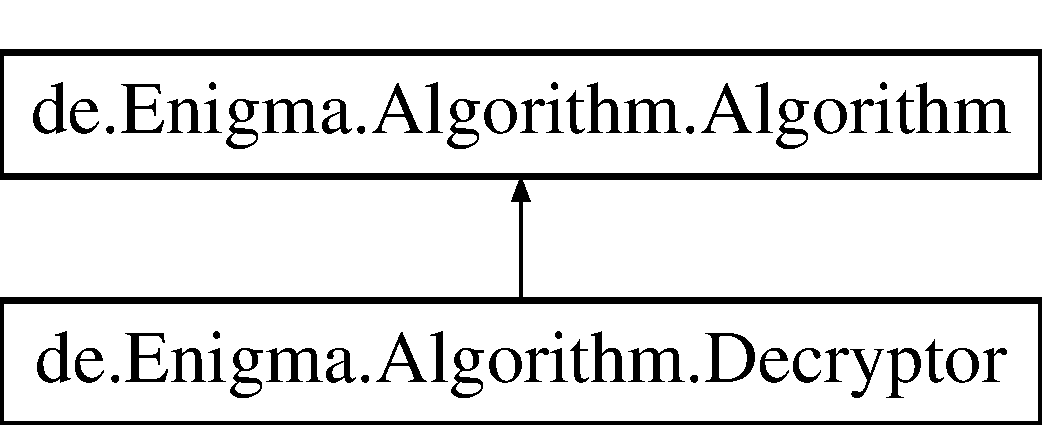
\includegraphics[height=2.000000cm]{classde_1_1_enigma_1_1_algorithm_1_1_decryptor}
\end{center}
\end{figure}
\subsection*{Protected Member Functions}
\begin{DoxyCompactItemize}
\item 
\mbox{\Hypertarget{classde_1_1_enigma_1_1_algorithm_1_1_decryptor_a7c62b71a4b7b74d3f4d3d2a79a5dbe83}\label{classde_1_1_enigma_1_1_algorithm_1_1_decryptor_a7c62b71a4b7b74d3f4d3d2a79a5dbe83}} 
void {\bfseries create\+Meta\+Data} ()
\end{DoxyCompactItemize}


The documentation for this class was generated from the following file\+:\begin{DoxyCompactItemize}
\item 
src/de/\+Enigma/\+Algorithm/Decryptor.\+java\end{DoxyCompactItemize}

\hypertarget{enumde_1_1_enigma_1_1_util_1_1_enums_1_1_e_alphabet}{}\section{de.\+Enigma.\+Util.\+Enums.\+E\+Alphabet Enum Reference}
\label{enumde_1_1_enigma_1_1_util_1_1_enums_1_1_e_alphabet}\index{de.\+Enigma.\+Util.\+Enums.\+E\+Alphabet@{de.\+Enigma.\+Util.\+Enums.\+E\+Alphabet}}


) Ein Enum, welches das \char`\"{}normale\char`\"{} Alphabet enthält  


\subsection*{Public Member Functions}
\begin{DoxyCompactItemize}
\item 
\mbox{\Hypertarget{enumde_1_1_enigma_1_1_util_1_1_enums_1_1_e_alphabet_a53563139df6bbf6ed8e642018a1d6baf}\label{enumde_1_1_enigma_1_1_util_1_1_enums_1_1_e_alphabet_a53563139df6bbf6ed8e642018a1d6baf}} 
{\bfseries E\+Alphabet} (char c, int i)
\item 
int \hyperlink{enumde_1_1_enigma_1_1_util_1_1_enums_1_1_e_alphabet_a9e9983168faaf9bb24090c3870ebbfa4}{get\+Index} ()
\item 
char \hyperlink{enumde_1_1_enigma_1_1_util_1_1_enums_1_1_e_alphabet_ab8be59c4d6bb5263147572911f75c5c5}{get\+As\+Char} ()
\end{DoxyCompactItemize}
\subsection*{Static Public Member Functions}
\begin{DoxyCompactItemize}
\item 
\mbox{\Hypertarget{enumde_1_1_enigma_1_1_util_1_1_enums_1_1_e_alphabet_ace27f61bd32f821d82345654b3b45bf8}\label{enumde_1_1_enigma_1_1_util_1_1_enums_1_1_e_alphabet_ace27f61bd32f821d82345654b3b45bf8}} 
static \hyperlink{enumde_1_1_enigma_1_1_util_1_1_enums_1_1_e_alphabet}{E\+Alphabet} {\bfseries get\+From\+Index} (int i)
\item 
static char \mbox{[}$\,$\mbox{]} \hyperlink{enumde_1_1_enigma_1_1_util_1_1_enums_1_1_e_alphabet_aebee015859ad2b6090c8ccf06fcdcd28}{get\+Alphabet} ()
\end{DoxyCompactItemize}
\subsection*{Public Attributes}
\begin{DoxyCompactItemize}
\item 
\mbox{\Hypertarget{enumde_1_1_enigma_1_1_util_1_1_enums_1_1_e_alphabet_aadc37deda02b68e773b3679972c4ec87}\label{enumde_1_1_enigma_1_1_util_1_1_enums_1_1_e_alphabet_aadc37deda02b68e773b3679972c4ec87}} 
{\bfseries A} =(\textquotesingle{}a\textquotesingle{},1)
\item 
\mbox{\Hypertarget{enumde_1_1_enigma_1_1_util_1_1_enums_1_1_e_alphabet_a4d00ed4b20b441ae95186a6a5ab152aa}\label{enumde_1_1_enigma_1_1_util_1_1_enums_1_1_e_alphabet_a4d00ed4b20b441ae95186a6a5ab152aa}} 
{\bfseries B} =(\textquotesingle{}b\textquotesingle{},2)
\item 
\mbox{\Hypertarget{enumde_1_1_enigma_1_1_util_1_1_enums_1_1_e_alphabet_a184ea708d1d370ce9df7ec97dd7e6cc7}\label{enumde_1_1_enigma_1_1_util_1_1_enums_1_1_e_alphabet_a184ea708d1d370ce9df7ec97dd7e6cc7}} 
{\bfseries C} =(\textquotesingle{}c\textquotesingle{},3)
\item 
\mbox{\Hypertarget{enumde_1_1_enigma_1_1_util_1_1_enums_1_1_e_alphabet_a02f68e03ddc9d53241aeb534ab6ce9d0}\label{enumde_1_1_enigma_1_1_util_1_1_enums_1_1_e_alphabet_a02f68e03ddc9d53241aeb534ab6ce9d0}} 
{\bfseries D} =(\textquotesingle{}d\textquotesingle{},4)
\item 
\mbox{\Hypertarget{enumde_1_1_enigma_1_1_util_1_1_enums_1_1_e_alphabet_a6e9e8350d5293a7cffe53072b62d52e1}\label{enumde_1_1_enigma_1_1_util_1_1_enums_1_1_e_alphabet_a6e9e8350d5293a7cffe53072b62d52e1}} 
{\bfseries E} =(\textquotesingle{}e\textquotesingle{},5)
\item 
\mbox{\Hypertarget{enumde_1_1_enigma_1_1_util_1_1_enums_1_1_e_alphabet_a31042332f54cc6e20bf6f141b0dfedd3}\label{enumde_1_1_enigma_1_1_util_1_1_enums_1_1_e_alphabet_a31042332f54cc6e20bf6f141b0dfedd3}} 
{\bfseries F} =(\textquotesingle{}f\textquotesingle{},6)
\item 
\mbox{\Hypertarget{enumde_1_1_enigma_1_1_util_1_1_enums_1_1_e_alphabet_ac8f18f28104667235a1b236c06cdfc0b}\label{enumde_1_1_enigma_1_1_util_1_1_enums_1_1_e_alphabet_ac8f18f28104667235a1b236c06cdfc0b}} 
{\bfseries G} =(\textquotesingle{}g\textquotesingle{},7)
\item 
\mbox{\Hypertarget{enumde_1_1_enigma_1_1_util_1_1_enums_1_1_e_alphabet_a939d94dc9d421f5e3d297792fac05250}\label{enumde_1_1_enigma_1_1_util_1_1_enums_1_1_e_alphabet_a939d94dc9d421f5e3d297792fac05250}} 
{\bfseries H} =(\textquotesingle{}h\textquotesingle{},8)
\item 
\mbox{\Hypertarget{enumde_1_1_enigma_1_1_util_1_1_enums_1_1_e_alphabet_a9a45bf45be94d6b9bf0a885fecc03c26}\label{enumde_1_1_enigma_1_1_util_1_1_enums_1_1_e_alphabet_a9a45bf45be94d6b9bf0a885fecc03c26}} 
{\bfseries I} =(\textquotesingle{}i\textquotesingle{},9)
\item 
\mbox{\Hypertarget{enumde_1_1_enigma_1_1_util_1_1_enums_1_1_e_alphabet_a983b2b628e246f46666070b5dfd59451}\label{enumde_1_1_enigma_1_1_util_1_1_enums_1_1_e_alphabet_a983b2b628e246f46666070b5dfd59451}} 
{\bfseries J} =(\textquotesingle{}j\textquotesingle{},10)
\item 
\mbox{\Hypertarget{enumde_1_1_enigma_1_1_util_1_1_enums_1_1_e_alphabet_a7207ddfb1f56aa1a0c8c103a2368b317}\label{enumde_1_1_enigma_1_1_util_1_1_enums_1_1_e_alphabet_a7207ddfb1f56aa1a0c8c103a2368b317}} 
{\bfseries K} =(\textquotesingle{}k\textquotesingle{},11)
\item 
\mbox{\Hypertarget{enumde_1_1_enigma_1_1_util_1_1_enums_1_1_e_alphabet_ae505df2771dec95db95bb9f58dd16cc0}\label{enumde_1_1_enigma_1_1_util_1_1_enums_1_1_e_alphabet_ae505df2771dec95db95bb9f58dd16cc0}} 
{\bfseries L} =(\textquotesingle{}l\textquotesingle{},12)
\item 
\mbox{\Hypertarget{enumde_1_1_enigma_1_1_util_1_1_enums_1_1_e_alphabet_aa05876adf2d8e6764a39678b3768a6fa}\label{enumde_1_1_enigma_1_1_util_1_1_enums_1_1_e_alphabet_aa05876adf2d8e6764a39678b3768a6fa}} 
{\bfseries M} =(\textquotesingle{}m\textquotesingle{},13)
\item 
\mbox{\Hypertarget{enumde_1_1_enigma_1_1_util_1_1_enums_1_1_e_alphabet_abadc57a4407a1fa5770338c9c30611ea}\label{enumde_1_1_enigma_1_1_util_1_1_enums_1_1_e_alphabet_abadc57a4407a1fa5770338c9c30611ea}} 
{\bfseries N} =(\textquotesingle{}n\textquotesingle{},14)
\item 
\mbox{\Hypertarget{enumde_1_1_enigma_1_1_util_1_1_enums_1_1_e_alphabet_a92527b58880ed92b4a3a4dda73c29c2c}\label{enumde_1_1_enigma_1_1_util_1_1_enums_1_1_e_alphabet_a92527b58880ed92b4a3a4dda73c29c2c}} 
{\bfseries O} =(\textquotesingle{}o\textquotesingle{},15)
\item 
\mbox{\Hypertarget{enumde_1_1_enigma_1_1_util_1_1_enums_1_1_e_alphabet_a6baae5bb203b4640f01f248e9179699a}\label{enumde_1_1_enigma_1_1_util_1_1_enums_1_1_e_alphabet_a6baae5bb203b4640f01f248e9179699a}} 
{\bfseries P} =(\textquotesingle{}p\textquotesingle{},16)
\item 
\mbox{\Hypertarget{enumde_1_1_enigma_1_1_util_1_1_enums_1_1_e_alphabet_af75afa8b032650404e2831847fff598d}\label{enumde_1_1_enigma_1_1_util_1_1_enums_1_1_e_alphabet_af75afa8b032650404e2831847fff598d}} 
{\bfseries Q} =(\textquotesingle{}q\textquotesingle{},17)
\item 
\mbox{\Hypertarget{enumde_1_1_enigma_1_1_util_1_1_enums_1_1_e_alphabet_a918dfe7e306075dcd949dec252479119}\label{enumde_1_1_enigma_1_1_util_1_1_enums_1_1_e_alphabet_a918dfe7e306075dcd949dec252479119}} 
{\bfseries R} =(\textquotesingle{}r\textquotesingle{},18)
\item 
\mbox{\Hypertarget{enumde_1_1_enigma_1_1_util_1_1_enums_1_1_e_alphabet_a66515c5d828336c80beee9365ebb959b}\label{enumde_1_1_enigma_1_1_util_1_1_enums_1_1_e_alphabet_a66515c5d828336c80beee9365ebb959b}} 
{\bfseries S} =(\textquotesingle{}s\textquotesingle{},19)
\item 
\mbox{\Hypertarget{enumde_1_1_enigma_1_1_util_1_1_enums_1_1_e_alphabet_ae6b3aa3b17636f20a92ad5c63d624d68}\label{enumde_1_1_enigma_1_1_util_1_1_enums_1_1_e_alphabet_ae6b3aa3b17636f20a92ad5c63d624d68}} 
{\bfseries T} =(\textquotesingle{}t\textquotesingle{},20)
\item 
\mbox{\Hypertarget{enumde_1_1_enigma_1_1_util_1_1_enums_1_1_e_alphabet_a3eba1a14de1faad0974c3a418e3ffd5e}\label{enumde_1_1_enigma_1_1_util_1_1_enums_1_1_e_alphabet_a3eba1a14de1faad0974c3a418e3ffd5e}} 
{\bfseries U} =(\textquotesingle{}u\textquotesingle{},21)
\item 
\mbox{\Hypertarget{enumde_1_1_enigma_1_1_util_1_1_enums_1_1_e_alphabet_a03fb18b6d07705f3b33a72b3e7b225ed}\label{enumde_1_1_enigma_1_1_util_1_1_enums_1_1_e_alphabet_a03fb18b6d07705f3b33a72b3e7b225ed}} 
{\bfseries V} =(\textquotesingle{}v\textquotesingle{},22)
\item 
\mbox{\Hypertarget{enumde_1_1_enigma_1_1_util_1_1_enums_1_1_e_alphabet_aa7bd693378c1e8962bc8da031e239271}\label{enumde_1_1_enigma_1_1_util_1_1_enums_1_1_e_alphabet_aa7bd693378c1e8962bc8da031e239271}} 
{\bfseries W} =(\textquotesingle{}w\textquotesingle{},23)
\item 
\mbox{\Hypertarget{enumde_1_1_enigma_1_1_util_1_1_enums_1_1_e_alphabet_afbb56f1d9386caabf0e9babbab0037a1}\label{enumde_1_1_enigma_1_1_util_1_1_enums_1_1_e_alphabet_afbb56f1d9386caabf0e9babbab0037a1}} 
{\bfseries X} =(\textquotesingle{}x\textquotesingle{},24)
\item 
\mbox{\Hypertarget{enumde_1_1_enigma_1_1_util_1_1_enums_1_1_e_alphabet_a537d00de4603dcc3d4b29cf5d681ed39}\label{enumde_1_1_enigma_1_1_util_1_1_enums_1_1_e_alphabet_a537d00de4603dcc3d4b29cf5d681ed39}} 
{\bfseries Y} =(\textquotesingle{}y\textquotesingle{},25)
\item 
\mbox{\Hypertarget{enumde_1_1_enigma_1_1_util_1_1_enums_1_1_e_alphabet_a804799235329692d5902df4c5c3b286a}\label{enumde_1_1_enigma_1_1_util_1_1_enums_1_1_e_alphabet_a804799235329692d5902df4c5c3b286a}} 
{\bfseries Z} =(\textquotesingle{}z\textquotesingle{},26)
\end{DoxyCompactItemize}


\subsection{Detailed Description}
) Ein Enum, welches das \char`\"{}normale\char`\"{} Alphabet enthält 

(\begin{DoxyAuthor}{Author}
Der\+Boss 
\end{DoxyAuthor}


\subsection{Member Function Documentation}
\mbox{\Hypertarget{enumde_1_1_enigma_1_1_util_1_1_enums_1_1_e_alphabet_aebee015859ad2b6090c8ccf06fcdcd28}\label{enumde_1_1_enigma_1_1_util_1_1_enums_1_1_e_alphabet_aebee015859ad2b6090c8ccf06fcdcd28}} 
\index{de\+::\+Enigma\+::\+Util\+::\+Enums\+::\+E\+Alphabet@{de\+::\+Enigma\+::\+Util\+::\+Enums\+::\+E\+Alphabet}!get\+Alphabet@{get\+Alphabet}}
\index{get\+Alphabet@{get\+Alphabet}!de\+::\+Enigma\+::\+Util\+::\+Enums\+::\+E\+Alphabet@{de\+::\+Enigma\+::\+Util\+::\+Enums\+::\+E\+Alphabet}}
\subsubsection{\texorpdfstring{get\+Alphabet()}{getAlphabet()}}
{\footnotesize\ttfamily static char \mbox{[}$\,$\mbox{]} de.\+Enigma.\+Util.\+Enums.\+E\+Alphabet.\+get\+Alphabet (\begin{DoxyParamCaption}{ }\end{DoxyParamCaption})\hspace{0.3cm}{\ttfamily [static]}}

\begin{DoxyReturn}{Returns}
Liefert das normale Alphabet als array zurück 
\end{DoxyReturn}
\mbox{\Hypertarget{enumde_1_1_enigma_1_1_util_1_1_enums_1_1_e_alphabet_ab8be59c4d6bb5263147572911f75c5c5}\label{enumde_1_1_enigma_1_1_util_1_1_enums_1_1_e_alphabet_ab8be59c4d6bb5263147572911f75c5c5}} 
\index{de\+::\+Enigma\+::\+Util\+::\+Enums\+::\+E\+Alphabet@{de\+::\+Enigma\+::\+Util\+::\+Enums\+::\+E\+Alphabet}!get\+As\+Char@{get\+As\+Char}}
\index{get\+As\+Char@{get\+As\+Char}!de\+::\+Enigma\+::\+Util\+::\+Enums\+::\+E\+Alphabet@{de\+::\+Enigma\+::\+Util\+::\+Enums\+::\+E\+Alphabet}}
\subsubsection{\texorpdfstring{get\+As\+Char()}{getAsChar()}}
{\footnotesize\ttfamily char de.\+Enigma.\+Util.\+Enums.\+E\+Alphabet.\+get\+As\+Char (\begin{DoxyParamCaption}{ }\end{DoxyParamCaption})}

\begin{DoxyReturn}{Returns}
Liefert den char dieses Eintrags 
\end{DoxyReturn}
\mbox{\Hypertarget{enumde_1_1_enigma_1_1_util_1_1_enums_1_1_e_alphabet_a9e9983168faaf9bb24090c3870ebbfa4}\label{enumde_1_1_enigma_1_1_util_1_1_enums_1_1_e_alphabet_a9e9983168faaf9bb24090c3870ebbfa4}} 
\index{de\+::\+Enigma\+::\+Util\+::\+Enums\+::\+E\+Alphabet@{de\+::\+Enigma\+::\+Util\+::\+Enums\+::\+E\+Alphabet}!get\+Index@{get\+Index}}
\index{get\+Index@{get\+Index}!de\+::\+Enigma\+::\+Util\+::\+Enums\+::\+E\+Alphabet@{de\+::\+Enigma\+::\+Util\+::\+Enums\+::\+E\+Alphabet}}
\subsubsection{\texorpdfstring{get\+Index()}{getIndex()}}
{\footnotesize\ttfamily int de.\+Enigma.\+Util.\+Enums.\+E\+Alphabet.\+get\+Index (\begin{DoxyParamCaption}{ }\end{DoxyParamCaption})}

\begin{DoxyReturn}{Returns}
Liefert den Index dieses Eintrags im Alphabet zurück 
\end{DoxyReturn}


The documentation for this enum was generated from the following file\+:\begin{DoxyCompactItemize}
\item 
src/de/\+Enigma/\+Util/Enums.\+java\end{DoxyCompactItemize}

\hypertarget{enumde_1_1_enigma_1_1_util_1_1_enums_1_1_e_mill}{}\section{de.\+Enigma.\+Util.\+Enums.\+E\+Mill Enum Reference}
\label{enumde_1_1_enigma_1_1_util_1_1_enums_1_1_e_mill}\index{de.\+Enigma.\+Util.\+Enums.\+E\+Mill@{de.\+Enigma.\+Util.\+Enums.\+E\+Mill}}


) Dieses Enum wird dazu verwendet, um die Instanzen der Walzen der Enigma anzusprechen, bzw. zwischen ihnen zu differenzieren  


\subsection*{Public Attributes}
\begin{DoxyCompactItemize}
\item 
\mbox{\Hypertarget{enumde_1_1_enigma_1_1_util_1_1_enums_1_1_e_mill_a1fe7c36a499e336421fff6bbfbdc2d1f}\label{enumde_1_1_enigma_1_1_util_1_1_enums_1_1_e_mill_a1fe7c36a499e336421fff6bbfbdc2d1f}} 
{\bfseries F\+I\+R\+S\+T\+\_\+\+M\+I\+LL}
\item 
\mbox{\Hypertarget{enumde_1_1_enigma_1_1_util_1_1_enums_1_1_e_mill_a5efd3b3ec74667db7d6b28bd8c02a9a9}\label{enumde_1_1_enigma_1_1_util_1_1_enums_1_1_e_mill_a5efd3b3ec74667db7d6b28bd8c02a9a9}} 
{\bfseries S\+E\+C\+O\+N\+D\+\_\+\+M\+I\+LL}
\item 
\mbox{\Hypertarget{enumde_1_1_enigma_1_1_util_1_1_enums_1_1_e_mill_ad80ebf2e777a7badefe1de9b4f267f69}\label{enumde_1_1_enigma_1_1_util_1_1_enums_1_1_e_mill_ad80ebf2e777a7badefe1de9b4f267f69}} 
{\bfseries T\+H\+I\+R\+D\+\_\+\+M\+I\+LL}
\end{DoxyCompactItemize}


\subsection{Detailed Description}
) Dieses Enum wird dazu verwendet, um die Instanzen der Walzen der Enigma anzusprechen, bzw. zwischen ihnen zu differenzieren 

(\begin{DoxyAuthor}{Author}
Der\+Boss 
\end{DoxyAuthor}


The documentation for this enum was generated from the following file\+:\begin{DoxyCompactItemize}
\item 
src/de/\+Enigma/\+Util/Enums.\+java\end{DoxyCompactItemize}

\hypertarget{enumde_1_1_enigma_1_1_util_1_1_enums_1_1_e_mill_alphabet}{}\section{de.\+Enigma.\+Util.\+Enums.\+E\+Mill\+Alphabet Enum Reference}
\label{enumde_1_1_enigma_1_1_util_1_1_enums_1_1_e_mill_alphabet}\index{de.\+Enigma.\+Util.\+Enums.\+E\+Mill\+Alphabet@{de.\+Enigma.\+Util.\+Enums.\+E\+Mill\+Alphabet}}


) Dieses Enum enthält hauptsächlich die Alphabete für die Walzen 1-\/5 und die Umkehrwalzen A,B,C, welche in der Enigma I verbaut wurden  


\subsection*{Public Member Functions}
\begin{DoxyCompactItemize}
\item 
\mbox{\Hypertarget{enumde_1_1_enigma_1_1_util_1_1_enums_1_1_e_mill_alphabet_a758a01583486a28c58814f4b9655d8e2}\label{enumde_1_1_enigma_1_1_util_1_1_enums_1_1_e_mill_alphabet_a758a01583486a28c58814f4b9655d8e2}} 
{\bfseries E\+Mill\+Alphabet} (String mill\+ID, char\mbox{[}$\,$\mbox{]} mill\+Phabet, char turn\+Marker)
\item 
char \hyperlink{enumde_1_1_enigma_1_1_util_1_1_enums_1_1_e_mill_alphabet_a0e912c02d1cc35b4ff6637674bcc7c58}{get\+Turn\+Marker} ()
\item 
char \mbox{[}$\,$\mbox{]} \hyperlink{enumde_1_1_enigma_1_1_util_1_1_enums_1_1_e_mill_alphabet_a42738303dfbfa63d512306b1102a93cf}{get\+Alphabet} ()
\item 
String \hyperlink{enumde_1_1_enigma_1_1_util_1_1_enums_1_1_e_mill_alphabet_a69675608ee623ace1204f2cd46483034}{get\+Mill\+ID} ()
\end{DoxyCompactItemize}
\subsection*{Public Attributes}
\begin{DoxyCompactItemize}
\item 
\mbox{\Hypertarget{enumde_1_1_enigma_1_1_util_1_1_enums_1_1_e_mill_alphabet_af8844c7143464e031fe91ae2f65f3fef}\label{enumde_1_1_enigma_1_1_util_1_1_enums_1_1_e_mill_alphabet_af8844c7143464e031fe91ae2f65f3fef}} 
{\bfseries I} =(\char`\"{}1\char`\"{}, new char\mbox{[}$\,$\mbox{]} \{\textquotesingle{}E\textquotesingle{},\textquotesingle{}K\textquotesingle{},\textquotesingle{}M\textquotesingle{},\textquotesingle{}F\textquotesingle{},\textquotesingle{}L\textquotesingle{},\textquotesingle{}G\textquotesingle{},\textquotesingle{}D\textquotesingle{},\textquotesingle{}Q\textquotesingle{},\textquotesingle{}V\textquotesingle{},\textquotesingle{}Z\textquotesingle{},\textquotesingle{}N\textquotesingle{},\textquotesingle{}T\textquotesingle{},\textquotesingle{}O\textquotesingle{},\textquotesingle{}W\textquotesingle{},\textquotesingle{}Y\textquotesingle{},\textquotesingle{}H\textquotesingle{},\textquotesingle{}X\textquotesingle{},\textquotesingle{}U\textquotesingle{},\textquotesingle{}S\textquotesingle{},\textquotesingle{}P\textquotesingle{},\textquotesingle{}A\textquotesingle{},\textquotesingle{}I\textquotesingle{},\textquotesingle{}B\textquotesingle{},\textquotesingle{}R\textquotesingle{},\textquotesingle{}C\textquotesingle{},\textquotesingle{}J\textquotesingle{}\}, \textquotesingle{}X\textquotesingle{})
\item 
\mbox{\Hypertarget{enumde_1_1_enigma_1_1_util_1_1_enums_1_1_e_mill_alphabet_a1b8bf26e36720f82afe92911ca386e5c}\label{enumde_1_1_enigma_1_1_util_1_1_enums_1_1_e_mill_alphabet_a1b8bf26e36720f82afe92911ca386e5c}} 
{\bfseries II} =(\char`\"{}2\char`\"{}, new char\mbox{[}$\,$\mbox{]} \{\textquotesingle{}A\textquotesingle{},\textquotesingle{}J\textquotesingle{},\textquotesingle{}D\textquotesingle{},\textquotesingle{}K\textquotesingle{},\textquotesingle{}S\textquotesingle{},\textquotesingle{}I\textquotesingle{},\textquotesingle{}R\textquotesingle{},\textquotesingle{}U\textquotesingle{},\textquotesingle{}X\textquotesingle{},\textquotesingle{}B\textquotesingle{},\textquotesingle{}L\textquotesingle{},\textquotesingle{}H\textquotesingle{},\textquotesingle{}W\textquotesingle{},\textquotesingle{}T\textquotesingle{},\textquotesingle{}M\textquotesingle{},\textquotesingle{}C\textquotesingle{},\textquotesingle{}Q\textquotesingle{},\textquotesingle{}G\textquotesingle{},\textquotesingle{}Z\textquotesingle{},\textquotesingle{}N\textquotesingle{},\textquotesingle{}P\textquotesingle{},\textquotesingle{}Y\textquotesingle{},\textquotesingle{}F\textquotesingle{},\textquotesingle{}V\textquotesingle{},\textquotesingle{}O\textquotesingle{},\textquotesingle{}E\textquotesingle{}\}, \textquotesingle{}S\textquotesingle{})
\item 
\mbox{\Hypertarget{enumde_1_1_enigma_1_1_util_1_1_enums_1_1_e_mill_alphabet_a572774577e69156f77f5e6cb98b72234}\label{enumde_1_1_enigma_1_1_util_1_1_enums_1_1_e_mill_alphabet_a572774577e69156f77f5e6cb98b72234}} 
{\bfseries I\+II} =(\char`\"{}3\char`\"{}, new char\mbox{[}$\,$\mbox{]} \{\textquotesingle{}B\textquotesingle{},\textquotesingle{}D\textquotesingle{},\textquotesingle{}F\textquotesingle{},\textquotesingle{}H\textquotesingle{},\textquotesingle{}J\textquotesingle{},\textquotesingle{}L\textquotesingle{},\textquotesingle{}C\textquotesingle{},\textquotesingle{}P\textquotesingle{},\textquotesingle{}R\textquotesingle{},\textquotesingle{}T\textquotesingle{},\textquotesingle{}X\textquotesingle{},\textquotesingle{}V\textquotesingle{},\textquotesingle{}Z\textquotesingle{},\textquotesingle{}N\textquotesingle{},\textquotesingle{}Y\textquotesingle{},\textquotesingle{}E\textquotesingle{},\textquotesingle{}I\textquotesingle{},\textquotesingle{}W\textquotesingle{},\textquotesingle{}G\textquotesingle{},\textquotesingle{}A\textquotesingle{},\textquotesingle{}K\textquotesingle{},\textquotesingle{}M\textquotesingle{},\textquotesingle{}U\textquotesingle{},\textquotesingle{}S\textquotesingle{},\textquotesingle{}Q\textquotesingle{},\textquotesingle{}O\textquotesingle{}\}, \textquotesingle{}M\textquotesingle{})
\item 
\mbox{\Hypertarget{enumde_1_1_enigma_1_1_util_1_1_enums_1_1_e_mill_alphabet_aeca0f5a2e979e7845ac07915e3c00bd6}\label{enumde_1_1_enigma_1_1_util_1_1_enums_1_1_e_mill_alphabet_aeca0f5a2e979e7845ac07915e3c00bd6}} 
{\bfseries IV} =(\char`\"{}4\char`\"{}, new char\mbox{[}$\,$\mbox{]} \{\textquotesingle{}E\textquotesingle{},\textquotesingle{}S\textquotesingle{},\textquotesingle{}O\textquotesingle{},\textquotesingle{}V\textquotesingle{},\textquotesingle{}P\textquotesingle{},\textquotesingle{}Z\textquotesingle{},\textquotesingle{}J\textquotesingle{},\textquotesingle{}A\textquotesingle{},\textquotesingle{}Y\textquotesingle{},\textquotesingle{}Q\textquotesingle{},\textquotesingle{}U\textquotesingle{},\textquotesingle{}I\textquotesingle{},\textquotesingle{}R\textquotesingle{},\textquotesingle{}H\textquotesingle{},\textquotesingle{}X\textquotesingle{},\textquotesingle{}L\textquotesingle{},\textquotesingle{}N\textquotesingle{},\textquotesingle{}F\textquotesingle{},\textquotesingle{}T\textquotesingle{},\textquotesingle{}G\textquotesingle{},\textquotesingle{}K\textquotesingle{},\textquotesingle{}D\textquotesingle{},\textquotesingle{}C\textquotesingle{},\textquotesingle{}M\textquotesingle{},\textquotesingle{}W\textquotesingle{},\textquotesingle{}B\textquotesingle{}\}, \textquotesingle{}Q\textquotesingle{})
\item 
\mbox{\Hypertarget{enumde_1_1_enigma_1_1_util_1_1_enums_1_1_e_mill_alphabet_aa26fea3741f0c38bf15204bbf0cba51d}\label{enumde_1_1_enigma_1_1_util_1_1_enums_1_1_e_mill_alphabet_aa26fea3741f0c38bf15204bbf0cba51d}} 
{\bfseries V} =(\char`\"{}5\char`\"{}, new char\mbox{[}$\,$\mbox{]} \{\textquotesingle{}V\textquotesingle{},\textquotesingle{}Z\textquotesingle{},\textquotesingle{}B\textquotesingle{},\textquotesingle{}R\textquotesingle{},\textquotesingle{}G\textquotesingle{},\textquotesingle{}I\textquotesingle{},\textquotesingle{}T\textquotesingle{},\textquotesingle{}Y\textquotesingle{},\textquotesingle{}U\textquotesingle{},\textquotesingle{}P\textquotesingle{},\textquotesingle{}S\textquotesingle{},\textquotesingle{}D\textquotesingle{},\textquotesingle{}N\textquotesingle{},\textquotesingle{}H\textquotesingle{},\textquotesingle{}L\textquotesingle{},\textquotesingle{}X\textquotesingle{},\textquotesingle{}A\textquotesingle{},\textquotesingle{}W\textquotesingle{},\textquotesingle{}M\textquotesingle{},\textquotesingle{}J\textquotesingle{},\textquotesingle{}Q\textquotesingle{},\textquotesingle{}O\textquotesingle{},\textquotesingle{}F\textquotesingle{},\textquotesingle{}E\textquotesingle{},\textquotesingle{}C\textquotesingle{},\textquotesingle{}K\textquotesingle{}\}, \textquotesingle{}K\textquotesingle{})
\item 
\mbox{\Hypertarget{enumde_1_1_enigma_1_1_util_1_1_enums_1_1_e_mill_alphabet_a506fed75dbe1428bfb4f863f4300cf20}\label{enumde_1_1_enigma_1_1_util_1_1_enums_1_1_e_mill_alphabet_a506fed75dbe1428bfb4f863f4300cf20}} 
{\bfseries U\+K\+W\+\_\+A} =(\char`\"{}A\char`\"{}, new char\mbox{[}$\,$\mbox{]} \{\textquotesingle{}E\textquotesingle{},\textquotesingle{}J\textquotesingle{},\textquotesingle{}M\textquotesingle{},\textquotesingle{}Z\textquotesingle{},\textquotesingle{}A\textquotesingle{},\textquotesingle{}L\textquotesingle{},\textquotesingle{}Y\textquotesingle{},\textquotesingle{}X\textquotesingle{},\textquotesingle{}V\textquotesingle{},\textquotesingle{}B\textquotesingle{},\textquotesingle{}W\textquotesingle{},\textquotesingle{}F\textquotesingle{},\textquotesingle{}C\textquotesingle{},\textquotesingle{}R\textquotesingle{},\textquotesingle{}Q\textquotesingle{},\textquotesingle{}U\textquotesingle{},\textquotesingle{}O\textquotesingle{},\textquotesingle{}N\textquotesingle{},\textquotesingle{}T\textquotesingle{},\textquotesingle{}S\textquotesingle{},\textquotesingle{}P\textquotesingle{},\textquotesingle{}I\textquotesingle{},\textquotesingle{}K\textquotesingle{},\textquotesingle{}H\textquotesingle{},\textquotesingle{}G\textquotesingle{},\textquotesingle{}D\textquotesingle{}\}, \textquotesingle{}?\textquotesingle{})
\item 
\mbox{\Hypertarget{enumde_1_1_enigma_1_1_util_1_1_enums_1_1_e_mill_alphabet_a0632fa145edc0305f2f9072e0595c3a7}\label{enumde_1_1_enigma_1_1_util_1_1_enums_1_1_e_mill_alphabet_a0632fa145edc0305f2f9072e0595c3a7}} 
{\bfseries U\+K\+W\+\_\+B} =(\char`\"{}B\char`\"{}, new char\mbox{[}$\,$\mbox{]} \{\textquotesingle{}Y\textquotesingle{},\textquotesingle{}R\textquotesingle{},\textquotesingle{}U\textquotesingle{},\textquotesingle{}H\textquotesingle{},\textquotesingle{}Q\textquotesingle{},\textquotesingle{}S\textquotesingle{},\textquotesingle{}L\textquotesingle{},\textquotesingle{}D\textquotesingle{},\textquotesingle{}P\textquotesingle{},\textquotesingle{}X\textquotesingle{},\textquotesingle{}N\textquotesingle{},\textquotesingle{}G\textquotesingle{},\textquotesingle{}O\textquotesingle{},\textquotesingle{}K\textquotesingle{},\textquotesingle{}M\textquotesingle{},\textquotesingle{}I\textquotesingle{},\textquotesingle{}E\textquotesingle{},\textquotesingle{}B\textquotesingle{},\textquotesingle{}F\textquotesingle{},\textquotesingle{}Z\textquotesingle{},\textquotesingle{}C\textquotesingle{},\textquotesingle{}W\textquotesingle{},\textquotesingle{}V\textquotesingle{},\textquotesingle{}J\textquotesingle{},\textquotesingle{}A\textquotesingle{},\textquotesingle{}T\textquotesingle{}\}, \textquotesingle{}?\textquotesingle{})
\item 
\mbox{\Hypertarget{enumde_1_1_enigma_1_1_util_1_1_enums_1_1_e_mill_alphabet_aa81d529de5c03186a6e9fb0c120cb08d}\label{enumde_1_1_enigma_1_1_util_1_1_enums_1_1_e_mill_alphabet_aa81d529de5c03186a6e9fb0c120cb08d}} 
{\bfseries U\+K\+W\+\_\+C} =(\char`\"{}C\char`\"{}, new char\mbox{[}$\,$\mbox{]} \{\textquotesingle{}F\textquotesingle{},\textquotesingle{}V\textquotesingle{},\textquotesingle{}P\textquotesingle{},\textquotesingle{}J\textquotesingle{},\textquotesingle{}I\textquotesingle{},\textquotesingle{}A\textquotesingle{},\textquotesingle{}O\textquotesingle{},\textquotesingle{}Y\textquotesingle{},\textquotesingle{}E\textquotesingle{},\textquotesingle{}D\textquotesingle{},\textquotesingle{}R\textquotesingle{},\textquotesingle{}Z\textquotesingle{},\textquotesingle{}X\textquotesingle{},\textquotesingle{}W\textquotesingle{},\textquotesingle{}G\textquotesingle{},\textquotesingle{}C\textquotesingle{},\textquotesingle{}T\textquotesingle{},\textquotesingle{}K\textquotesingle{},\textquotesingle{}U\textquotesingle{},\textquotesingle{}Q\textquotesingle{},\textquotesingle{}S\textquotesingle{},\textquotesingle{}B\textquotesingle{},\textquotesingle{}N\textquotesingle{},\textquotesingle{}M\textquotesingle{},\textquotesingle{}H\textquotesingle{},\textquotesingle{}L\textquotesingle{}\}, \textquotesingle{}?\textquotesingle{})
\end{DoxyCompactItemize}


\subsection{Detailed Description}
) Dieses Enum enthält hauptsächlich die Alphabete für die Walzen 1-\/5 und die Umkehrwalzen A,B,C, welche in der Enigma I verbaut wurden 

(\begin{DoxyAuthor}{Author}
Der\+Boss 
\end{DoxyAuthor}


\subsection{Member Function Documentation}
\mbox{\Hypertarget{enumde_1_1_enigma_1_1_util_1_1_enums_1_1_e_mill_alphabet_a42738303dfbfa63d512306b1102a93cf}\label{enumde_1_1_enigma_1_1_util_1_1_enums_1_1_e_mill_alphabet_a42738303dfbfa63d512306b1102a93cf}} 
\index{de\+::\+Enigma\+::\+Util\+::\+Enums\+::\+E\+Mill\+Alphabet@{de\+::\+Enigma\+::\+Util\+::\+Enums\+::\+E\+Mill\+Alphabet}!get\+Alphabet@{get\+Alphabet}}
\index{get\+Alphabet@{get\+Alphabet}!de\+::\+Enigma\+::\+Util\+::\+Enums\+::\+E\+Mill\+Alphabet@{de\+::\+Enigma\+::\+Util\+::\+Enums\+::\+E\+Mill\+Alphabet}}
\subsubsection{\texorpdfstring{get\+Alphabet()}{getAlphabet()}}
{\footnotesize\ttfamily char \mbox{[}$\,$\mbox{]} de.\+Enigma.\+Util.\+Enums.\+E\+Mill\+Alphabet.\+get\+Alphabet (\begin{DoxyParamCaption}{ }\end{DoxyParamCaption})}

\begin{DoxyReturn}{Returns}
Liefert das verwendete Alphabet dieser Walze als char Array zurück 
\end{DoxyReturn}
\mbox{\Hypertarget{enumde_1_1_enigma_1_1_util_1_1_enums_1_1_e_mill_alphabet_a69675608ee623ace1204f2cd46483034}\label{enumde_1_1_enigma_1_1_util_1_1_enums_1_1_e_mill_alphabet_a69675608ee623ace1204f2cd46483034}} 
\index{de\+::\+Enigma\+::\+Util\+::\+Enums\+::\+E\+Mill\+Alphabet@{de\+::\+Enigma\+::\+Util\+::\+Enums\+::\+E\+Mill\+Alphabet}!get\+Mill\+ID@{get\+Mill\+ID}}
\index{get\+Mill\+ID@{get\+Mill\+ID}!de\+::\+Enigma\+::\+Util\+::\+Enums\+::\+E\+Mill\+Alphabet@{de\+::\+Enigma\+::\+Util\+::\+Enums\+::\+E\+Mill\+Alphabet}}
\subsubsection{\texorpdfstring{get\+Mill\+I\+D()}{getMillID()}}
{\footnotesize\ttfamily String de.\+Enigma.\+Util.\+Enums.\+E\+Mill\+Alphabet.\+get\+Mill\+ID (\begin{DoxyParamCaption}{ }\end{DoxyParamCaption})}

\begin{DoxyReturn}{Returns}
Liefert die \textquotesingle{}ID\textquotesingle{} dieser Walze zurück. 1-\/5\+: Walzen 1-\/5; A,B,C\+: Umkehrwalzen A,B,C 
\end{DoxyReturn}
\mbox{\Hypertarget{enumde_1_1_enigma_1_1_util_1_1_enums_1_1_e_mill_alphabet_a0e912c02d1cc35b4ff6637674bcc7c58}\label{enumde_1_1_enigma_1_1_util_1_1_enums_1_1_e_mill_alphabet_a0e912c02d1cc35b4ff6637674bcc7c58}} 
\index{de\+::\+Enigma\+::\+Util\+::\+Enums\+::\+E\+Mill\+Alphabet@{de\+::\+Enigma\+::\+Util\+::\+Enums\+::\+E\+Mill\+Alphabet}!get\+Turn\+Marker@{get\+Turn\+Marker}}
\index{get\+Turn\+Marker@{get\+Turn\+Marker}!de\+::\+Enigma\+::\+Util\+::\+Enums\+::\+E\+Mill\+Alphabet@{de\+::\+Enigma\+::\+Util\+::\+Enums\+::\+E\+Mill\+Alphabet}}
\subsubsection{\texorpdfstring{get\+Turn\+Marker()}{getTurnMarker()}}
{\footnotesize\ttfamily char de.\+Enigma.\+Util.\+Enums.\+E\+Mill\+Alphabet.\+get\+Turn\+Marker (\begin{DoxyParamCaption}{ }\end{DoxyParamCaption})}

\begin{DoxyReturn}{Returns}
Liefert den Buchstaben zurück, an welchem diese Walze ihre Übertragskerbe hat. Ist dieser \textquotesingle{}?\textquotesingle{}, so ist diese Walze eine Umkehrwalze, welche keine Übertragskerbe besitzt 
\end{DoxyReturn}


The documentation for this enum was generated from the following file\+:\begin{DoxyCompactItemize}
\item 
src/de/\+Enigma/\+Util/Enums.\+java\end{DoxyCompactItemize}

\hypertarget{enumde_1_1_enigma_1_1_util_1_1_enums_1_1_e_mode}{}\section{de.\+Enigma.\+Util.\+Enums.\+E\+Mode Enum Reference}
\label{enumde_1_1_enigma_1_1_util_1_1_enums_1_1_e_mode}\index{de.\+Enigma.\+Util.\+Enums.\+E\+Mode@{de.\+Enigma.\+Util.\+Enums.\+E\+Mode}}


) Benutzt für die Übergabe des gewählten Modus der Enigma  


\subsection*{Public Attributes}
\begin{DoxyCompactItemize}
\item 
\mbox{\Hypertarget{enumde_1_1_enigma_1_1_util_1_1_enums_1_1_e_mode_a2506d5250eaa2bc60de3fec91ff5805e}\label{enumde_1_1_enigma_1_1_util_1_1_enums_1_1_e_mode_a2506d5250eaa2bc60de3fec91ff5805e}} 
{\bfseries E\+N\+C\+R\+Y\+PT}
\end{DoxyCompactItemize}


\subsection{Detailed Description}
) Benutzt für die Übergabe des gewählten Modus der Enigma 

(\begin{DoxyAuthor}{Author}
Der\+Boss 
\end{DoxyAuthor}


The documentation for this enum was generated from the following file\+:\begin{DoxyCompactItemize}
\item 
src/de/\+Enigma/\+Util/Enums.\+java\end{DoxyCompactItemize}

\hypertarget{classde_1_1_enigma_1_1_algorithm_1_1_encryptor}{}\section{de.\+Enigma.\+Algorithm.\+Encryptor Class Reference}
\label{classde_1_1_enigma_1_1_algorithm_1_1_encryptor}\index{de.\+Enigma.\+Algorithm.\+Encryptor@{de.\+Enigma.\+Algorithm.\+Encryptor}}
Inheritance diagram for de.\+Enigma.\+Algorithm.\+Encryptor\+:\begin{figure}[H]
\begin{center}
\leavevmode
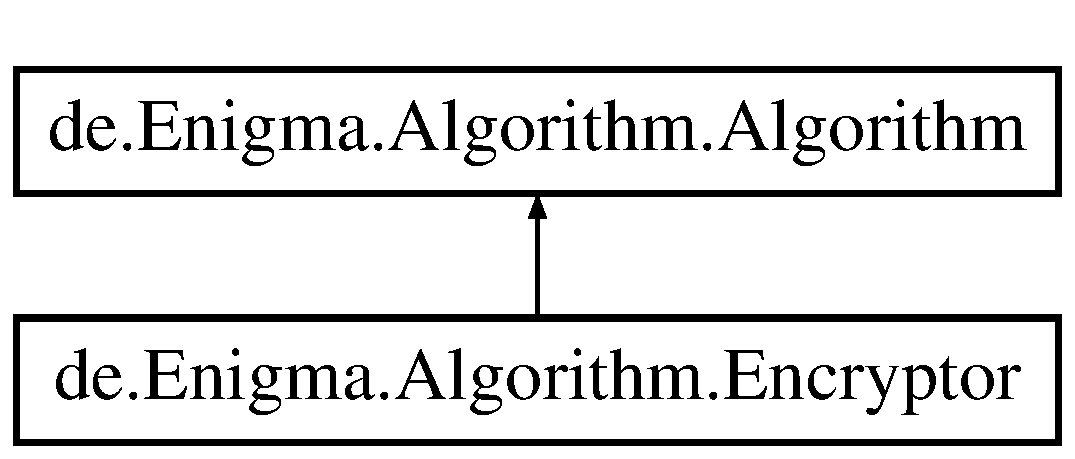
\includegraphics[height=2.000000cm]{classde_1_1_enigma_1_1_algorithm_1_1_encryptor}
\end{center}
\end{figure}
\subsection*{Protected Member Functions}
\begin{DoxyCompactItemize}
\item 
\mbox{\Hypertarget{classde_1_1_enigma_1_1_algorithm_1_1_encryptor_a8372de0c96311b2fce4d79c4df2b0cda}\label{classde_1_1_enigma_1_1_algorithm_1_1_encryptor_a8372de0c96311b2fce4d79c4df2b0cda}} 
void {\bfseries create\+Meta\+Data} ()
\end{DoxyCompactItemize}


The documentation for this class was generated from the following file\+:\begin{DoxyCompactItemize}
\item 
src/de/\+Enigma/\+Algorithm/Encryptor.\+java\end{DoxyCompactItemize}

\hypertarget{classde_1_1_enigma_1_1_algorithm_1_1_enigma_config}{}\section{de.\+Enigma.\+Algorithm.\+Enigma\+Config Class Reference}
\label{classde_1_1_enigma_1_1_algorithm_1_1_enigma_config}\index{de.\+Enigma.\+Algorithm.\+Enigma\+Config@{de.\+Enigma.\+Algorithm.\+Enigma\+Config}}


) Klasse, welche essenziell für die Verschlüsselung ist (  


\subsection*{Public Member Functions}
\begin{DoxyCompactItemize}
\item 
\hyperlink{classde_1_1_enigma_1_1_algorithm_1_1_enigma_config_aa6eee4a7c5ca96c781a75b4de0ae8436}{Enigma\+Config} ()
\item 
\mbox{\Hypertarget{classde_1_1_enigma_1_1_algorithm_1_1_enigma_config_a2788ae04b5cea34f7193e486ced93f21}\label{classde_1_1_enigma_1_1_algorithm_1_1_enigma_config_a2788ae04b5cea34f7193e486ced93f21}} 
char {\bfseries encrypt\+Letter} (char letter)
\end{DoxyCompactItemize}


\subsection{Detailed Description}
) Klasse, welche essenziell für die Verschlüsselung ist ( 

(

) Enthält eine Hash\+Map, welche das \char`\"{}\+Steckbrett\char`\"{} realisiert (

) Enthält die Instanzen der Walzen, welche benutzt werden

\begin{DoxyAuthor}{Author}
Der\+Boss 
\end{DoxyAuthor}


\subsection{Constructor \& Destructor Documentation}
\mbox{\Hypertarget{classde_1_1_enigma_1_1_algorithm_1_1_enigma_config_aa6eee4a7c5ca96c781a75b4de0ae8436}\label{classde_1_1_enigma_1_1_algorithm_1_1_enigma_config_aa6eee4a7c5ca96c781a75b4de0ae8436}} 
\index{de\+::\+Enigma\+::\+Algorithm\+::\+Enigma\+Config@{de\+::\+Enigma\+::\+Algorithm\+::\+Enigma\+Config}!Enigma\+Config@{Enigma\+Config}}
\index{Enigma\+Config@{Enigma\+Config}!de\+::\+Enigma\+::\+Algorithm\+::\+Enigma\+Config@{de\+::\+Enigma\+::\+Algorithm\+::\+Enigma\+Config}}
\subsubsection{\texorpdfstring{Enigma\+Config()}{EnigmaConfig()}}
{\footnotesize\ttfamily de.\+Enigma.\+Algorithm.\+Enigma\+Config.\+Enigma\+Config (\begin{DoxyParamCaption}{ }\end{DoxyParamCaption})}

Constructor, erzeugt die Instanzen der Walzen und das Steckbrett anhand des Schlüssels 

The documentation for this class was generated from the following file\+:\begin{DoxyCompactItemize}
\item 
src/de/\+Enigma/\+Algorithm/Enigma\+Config.\+java\end{DoxyCompactItemize}

\hypertarget{classde_1_1_enigma_1_1_util_1_1_enums}{}\section{de.\+Enigma.\+Util.\+Enums Class Reference}
\label{classde_1_1_enigma_1_1_util_1_1_enums}\index{de.\+Enigma.\+Util.\+Enums@{de.\+Enigma.\+Util.\+Enums}}


) Klasse, welche verschiedene \hyperlink{classde_1_1_enigma_1_1_util_1_1_enums}{Enums} enthält, welche verschiedene Aufgaben erfüllen  


\subsection*{Classes}
\begin{DoxyCompactItemize}
\item 
enum \hyperlink{enumde_1_1_enigma_1_1_util_1_1_enums_1_1_e_alphabet}{E\+Alphabet}
\begin{DoxyCompactList}\small\item\em ) Ein Enum, welches das \char`\"{}normale\char`\"{} Alphabet enthält \end{DoxyCompactList}\item 
enum \hyperlink{enumde_1_1_enigma_1_1_util_1_1_enums_1_1_e_mill}{E\+Mill}
\begin{DoxyCompactList}\small\item\em ) Dieses Enum wird dazu verwendet, um die Instanzen der Walzen der Enigma anzusprechen, bzw. zwischen ihnen zu differenzieren \end{DoxyCompactList}\item 
enum \hyperlink{enumde_1_1_enigma_1_1_util_1_1_enums_1_1_e_mill_alphabet}{E\+Mill\+Alphabet}
\begin{DoxyCompactList}\small\item\em ) Dieses Enum enthält hauptsächlich die Alphabete für die Walzen 1-\/5 und die Umkehrwalzen A,B,C, welche in der Enigma I verbaut wurden \end{DoxyCompactList}\item 
enum \hyperlink{enumde_1_1_enigma_1_1_util_1_1_enums_1_1_e_mode}{E\+Mode}
\begin{DoxyCompactList}\small\item\em ) Benutzt für die Übergabe des gewählten Modus der Enigma \end{DoxyCompactList}\end{DoxyCompactItemize}


\subsection{Detailed Description}
) Klasse, welche verschiedene \hyperlink{classde_1_1_enigma_1_1_util_1_1_enums}{Enums} enthält, welche verschiedene Aufgaben erfüllen 

(\begin{DoxyAuthor}{Author}
Der\+Boss 
\end{DoxyAuthor}


The documentation for this class was generated from the following file\+:\begin{DoxyCompactItemize}
\item 
src/de/\+Enigma/\+Util/Enums.\+java\end{DoxyCompactItemize}

\hypertarget{classde_1_1_enigma_1_1_util_1_1_file_handler}{}\section{de.\+Enigma.\+Util.\+File\+Handler Class Reference}
\label{classde_1_1_enigma_1_1_util_1_1_file_handler}\index{de.\+Enigma.\+Util.\+File\+Handler@{de.\+Enigma.\+Util.\+File\+Handler}}
\subsection*{Public Member Functions}
\begin{DoxyCompactItemize}
\item 
\mbox{\Hypertarget{classde_1_1_enigma_1_1_util_1_1_file_handler_a79a8f6db44470265e74f7b99c9894a14}\label{classde_1_1_enigma_1_1_util_1_1_file_handler_a79a8f6db44470265e74f7b99c9894a14}} 
void {\bfseries append\+Char} (char letter)
\item 
\mbox{\Hypertarget{classde_1_1_enigma_1_1_util_1_1_file_handler_a9683e0497063a3832805e4b516033d1b}\label{classde_1_1_enigma_1_1_util_1_1_file_handler_a9683e0497063a3832805e4b516033d1b}} 
void {\bfseries force\+Write} ()
\item 
\mbox{\Hypertarget{classde_1_1_enigma_1_1_util_1_1_file_handler_ace397e02b23a30baa565ec14395cef14}\label{classde_1_1_enigma_1_1_util_1_1_file_handler_ace397e02b23a30baa565ec14395cef14}} 
String {\bfseries get\+P\+A\+TH} ()
\end{DoxyCompactItemize}


The documentation for this class was generated from the following file\+:\begin{DoxyCompactItemize}
\item 
src/de/\+Enigma/\+Util/File\+Handler.\+java\end{DoxyCompactItemize}

\hypertarget{classde_1_1_enigma_1_1_u_i_1_1_g_u_i}{}\section{de.\+Enigma.\+U\+I.\+G\+UI Class Reference}
\label{classde_1_1_enigma_1_1_u_i_1_1_g_u_i}\index{de.\+Enigma.\+U\+I.\+G\+UI@{de.\+Enigma.\+U\+I.\+G\+UI}}
\subsection*{Public Member Functions}
\begin{DoxyCompactItemize}
\item 
\hyperlink{classde_1_1_enigma_1_1_u_i_1_1_g_u_i_ac98b39fcda7d523f32565a14ca1b8487}{G\+UI} (\hyperlink{classde_1_1_enigma_1_1_core_1_1_main}{Main} m)
\item 
\mbox{\Hypertarget{classde_1_1_enigma_1_1_u_i_1_1_g_u_i_af18e71a09d8ddb27e1a509e71ca3907f}\label{classde_1_1_enigma_1_1_u_i_1_1_g_u_i_af18e71a09d8ddb27e1a509e71ca3907f}} 
void {\bfseries show} ()
\item 
\mbox{\Hypertarget{classde_1_1_enigma_1_1_u_i_1_1_g_u_i_a34b0741a65eb5dd157afeb9ecdc17252}\label{classde_1_1_enigma_1_1_u_i_1_1_g_u_i_a34b0741a65eb5dd157afeb9ecdc17252}} 
void {\bfseries hide} ()
\item 
\mbox{\Hypertarget{classde_1_1_enigma_1_1_u_i_1_1_g_u_i_a298bbca8a9e094757b7443530b181c37}\label{classde_1_1_enigma_1_1_u_i_1_1_g_u_i_a298bbca8a9e094757b7443530b181c37}} 
void {\bfseries on\+Finished} ()
\end{DoxyCompactItemize}


\subsection{Constructor \& Destructor Documentation}
\mbox{\Hypertarget{classde_1_1_enigma_1_1_u_i_1_1_g_u_i_ac98b39fcda7d523f32565a14ca1b8487}\label{classde_1_1_enigma_1_1_u_i_1_1_g_u_i_ac98b39fcda7d523f32565a14ca1b8487}} 
\index{de\+::\+Enigma\+::\+U\+I\+::\+G\+UI@{de\+::\+Enigma\+::\+U\+I\+::\+G\+UI}!G\+UI@{G\+UI}}
\index{G\+UI@{G\+UI}!de\+::\+Enigma\+::\+U\+I\+::\+G\+UI@{de\+::\+Enigma\+::\+U\+I\+::\+G\+UI}}
\subsubsection{\texorpdfstring{G\+U\+I()}{GUI()}}
{\footnotesize\ttfamily de.\+Enigma.\+U\+I.\+G\+U\+I.\+G\+UI (\begin{DoxyParamCaption}\item[{\hyperlink{classde_1_1_enigma_1_1_core_1_1_main}{Main}}]{m }\end{DoxyParamCaption})}

Create the application. 

The documentation for this class was generated from the following file\+:\begin{DoxyCompactItemize}
\item 
src/de/\+Enigma/\+U\+I/G\+U\+I.\+java\end{DoxyCompactItemize}

\hypertarget{classde_1_1_enigma_1_1_core_1_1_log}{}\section{de.\+Enigma.\+Core.\+Log Class Reference}
\label{classde_1_1_enigma_1_1_core_1_1_log}\index{de.\+Enigma.\+Core.\+Log@{de.\+Enigma.\+Core.\+Log}}


) Logger Klasse die eine in C++ geschriebene .dll einbindet, um die Logs zu schreiben (  


\subsection*{Public Member Functions}
\begin{DoxyCompactItemize}
\item 
void \hyperlink{classde_1_1_enigma_1_1_core_1_1_log_a98177adb81490a58cdb21b365e71f290}{i} (String class\+Name, String method\+Name, String info)
\item 
void \hyperlink{classde_1_1_enigma_1_1_core_1_1_log_a2c72582bc2dd2fd464f5a4cb7109f894}{w} (String class\+Name, String method\+Name, String warning)
\item 
void \hyperlink{classde_1_1_enigma_1_1_core_1_1_log_a402f5a4a3b918b178cf711f02eb6f67a}{e} (String class\+Name, String method\+Name, String error)
\end{DoxyCompactItemize}
\subsection*{Static Public Member Functions}
\begin{DoxyCompactItemize}
\item 
static \hyperlink{classde_1_1_enigma_1_1_core_1_1_log}{Log} \hyperlink{classde_1_1_enigma_1_1_core_1_1_log_a06d2a4076d1150b2743351602fbfbc82}{get\+Logger} ()
\end{DoxyCompactItemize}


\subsection{Detailed Description}
) Logger Klasse die eine in C++ geschriebene .dll einbindet, um die Logs zu schreiben ( 

(

) Realisiert als Singleton -\/$>$ nur eine Instanz pro Programminstanz (

) Zugriff über \hyperlink{classde_1_1_enigma_1_1_core_1_1_log_a06d2a4076d1150b2743351602fbfbc82}{get\+Logger()} Methode von überall aus möglich

\begin{DoxyAuthor}{Author}
Nikolai 
\end{DoxyAuthor}


\subsection{Member Function Documentation}
\mbox{\Hypertarget{classde_1_1_enigma_1_1_core_1_1_log_a402f5a4a3b918b178cf711f02eb6f67a}\label{classde_1_1_enigma_1_1_core_1_1_log_a402f5a4a3b918b178cf711f02eb6f67a}} 
\index{de\+::\+Enigma\+::\+Core\+::\+Log@{de\+::\+Enigma\+::\+Core\+::\+Log}!e@{e}}
\index{e@{e}!de\+::\+Enigma\+::\+Core\+::\+Log@{de\+::\+Enigma\+::\+Core\+::\+Log}}
\subsubsection{\texorpdfstring{e()}{e()}}
{\footnotesize\ttfamily void de.\+Enigma.\+Core.\+Log.\+e (\begin{DoxyParamCaption}\item[{String}]{class\+Name,  }\item[{String}]{method\+Name,  }\item[{String}]{error }\end{DoxyParamCaption})}

Error Logeintrag\+: erstellt über die .dll einen Error-\/\+Log der über kritische Fehler innerhalb der Anwendung informieren soll


\begin{DoxyParams}{Parameters}
{\em class\+Name} & Name der Klasse von der der Aufruf erfolgt ist \\
\hline
{\em method\+Name} & Name der Methode von der der Aufruf erfolgt ist \\
\hline
{\em error} & Error Nachricht, die vom Logger geloggt werden soll \\
\hline
\end{DoxyParams}
\mbox{\Hypertarget{classde_1_1_enigma_1_1_core_1_1_log_a06d2a4076d1150b2743351602fbfbc82}\label{classde_1_1_enigma_1_1_core_1_1_log_a06d2a4076d1150b2743351602fbfbc82}} 
\index{de\+::\+Enigma\+::\+Core\+::\+Log@{de\+::\+Enigma\+::\+Core\+::\+Log}!get\+Logger@{get\+Logger}}
\index{get\+Logger@{get\+Logger}!de\+::\+Enigma\+::\+Core\+::\+Log@{de\+::\+Enigma\+::\+Core\+::\+Log}}
\subsubsection{\texorpdfstring{get\+Logger()}{getLogger()}}
{\footnotesize\ttfamily static \hyperlink{classde_1_1_enigma_1_1_core_1_1_log}{Log} de.\+Enigma.\+Core.\+Log.\+get\+Logger (\begin{DoxyParamCaption}{ }\end{DoxyParamCaption})\hspace{0.3cm}{\ttfamily [static]}}

(

) erstellt ein Singleton Objekt, sobald die Instanz benötigt wird (

) Das stellt sicher, dass es nur einen Logger gibt und dieser von allen Objekten von überall aus genutzt werden kann.

\begin{DoxyReturn}{Returns}
gibt das logger Singelton Objekt zurück 
\end{DoxyReturn}
\mbox{\Hypertarget{classde_1_1_enigma_1_1_core_1_1_log_a98177adb81490a58cdb21b365e71f290}\label{classde_1_1_enigma_1_1_core_1_1_log_a98177adb81490a58cdb21b365e71f290}} 
\index{de\+::\+Enigma\+::\+Core\+::\+Log@{de\+::\+Enigma\+::\+Core\+::\+Log}!i@{i}}
\index{i@{i}!de\+::\+Enigma\+::\+Core\+::\+Log@{de\+::\+Enigma\+::\+Core\+::\+Log}}
\subsubsection{\texorpdfstring{i()}{i()}}
{\footnotesize\ttfamily void de.\+Enigma.\+Core.\+Log.\+i (\begin{DoxyParamCaption}\item[{String}]{class\+Name,  }\item[{String}]{method\+Name,  }\item[{String}]{info }\end{DoxyParamCaption})}

Info Logeintrag\+: erstellt über die .dll einen Info-\/\+Log der über Vorgänge innerhalb der Anwendung informieren soll


\begin{DoxyParams}{Parameters}
{\em class\+Name} & Name der Klasse von der der Aufruf erfolgt ist \\
\hline
{\em method\+Name} & Name der Methode von der der Aufruf erfolgt ist \\
\hline
{\em info} & Info Nachricht, die vom Logger geloggt werden soll \\
\hline
\end{DoxyParams}
\mbox{\Hypertarget{classde_1_1_enigma_1_1_core_1_1_log_a2c72582bc2dd2fd464f5a4cb7109f894}\label{classde_1_1_enigma_1_1_core_1_1_log_a2c72582bc2dd2fd464f5a4cb7109f894}} 
\index{de\+::\+Enigma\+::\+Core\+::\+Log@{de\+::\+Enigma\+::\+Core\+::\+Log}!w@{w}}
\index{w@{w}!de\+::\+Enigma\+::\+Core\+::\+Log@{de\+::\+Enigma\+::\+Core\+::\+Log}}
\subsubsection{\texorpdfstring{w()}{w()}}
{\footnotesize\ttfamily void de.\+Enigma.\+Core.\+Log.\+w (\begin{DoxyParamCaption}\item[{String}]{class\+Name,  }\item[{String}]{method\+Name,  }\item[{String}]{warning }\end{DoxyParamCaption})}

Warning Logeintrag\+: erstellt über die .dll einen Warning-\/\+Log der über potentiell gefährliche Vorgänge innerhalb der Anwendung informieren soll


\begin{DoxyParams}{Parameters}
{\em class\+Name} & Name der Klasse von der der Aufruf erfolgt ist \\
\hline
{\em method\+Name} & Name der Methode von der der Aufruf erfolgt ist \\
\hline
{\em warning} & Warning Nachricht, die vom Logger geloggt werden soll \\
\hline
\end{DoxyParams}


The documentation for this class was generated from the following file\+:\begin{DoxyCompactItemize}
\item 
src/de/\+Enigma/\+Core/Log.\+java\end{DoxyCompactItemize}

\hypertarget{classde_1_1_enigma_1_1_core_1_1_main}{}\section{de.\+Enigma.\+Core.\+Main Class Reference}
\label{classde_1_1_enigma_1_1_core_1_1_main}\index{de.\+Enigma.\+Core.\+Main@{de.\+Enigma.\+Core.\+Main}}
\subsection*{Public Member Functions}
\begin{DoxyCompactItemize}
\item 
\mbox{\Hypertarget{classde_1_1_enigma_1_1_core_1_1_main_a310209f66ddc6fe17114f8a1f9c663ad}\label{classde_1_1_enigma_1_1_core_1_1_main_a310209f66ddc6fe17114f8a1f9c663ad}} 
void {\bfseries btn\+Ok\+Clicked} (String text, String key, boolean encrypt)
\item 
\mbox{\Hypertarget{classde_1_1_enigma_1_1_core_1_1_main_afc8fb7733ef95bfd1e2d9ec1ece359bd}\label{classde_1_1_enigma_1_1_core_1_1_main_afc8fb7733ef95bfd1e2d9ec1ece359bd}} 
void {\bfseries btn\+Cancel\+Clicked} ()
\item 
\mbox{\Hypertarget{classde_1_1_enigma_1_1_core_1_1_main_a96ef5b0aee61943c2262e1af9c058cda}\label{classde_1_1_enigma_1_1_core_1_1_main_a96ef5b0aee61943c2262e1af9c058cda}} 
\hyperlink{classde_1_1_enigma_1_1_util_1_1_file_handler}{File\+Handler} {\bfseries get\+File\+Handler} ()
\end{DoxyCompactItemize}
\subsection*{Static Public Member Functions}
\begin{DoxyCompactItemize}
\item 
\mbox{\Hypertarget{classde_1_1_enigma_1_1_core_1_1_main_a4559f91709b046a087e2a20cce660464}\label{classde_1_1_enigma_1_1_core_1_1_main_a4559f91709b046a087e2a20cce660464}} 
static void {\bfseries main} (String\mbox{[}$\,$\mbox{]} args)
\end{DoxyCompactItemize}


The documentation for this class was generated from the following file\+:\begin{DoxyCompactItemize}
\item 
src/de/\+Enigma/\+Core/Main.\+java\end{DoxyCompactItemize}

\hypertarget{classde_1_1_enigma_1_1_algorithm_1_1_mill}{}\section{de.\+Enigma.\+Algorithm.\+Mill Class Reference}
\label{classde_1_1_enigma_1_1_algorithm_1_1_mill}\index{de.\+Enigma.\+Algorithm.\+Mill@{de.\+Enigma.\+Algorithm.\+Mill}}


) Walzen Klasse, welche eine Walze der Enigma darstellt (  


\subsection*{Public Member Functions}
\begin{DoxyCompactItemize}
\item 
\hyperlink{classde_1_1_enigma_1_1_algorithm_1_1_mill_a51ac880f27208e0762445a6e6bce24a0}{Mill} (int indx, char start\+Pos, \hyperlink{enumde_1_1_enigma_1_1_util_1_1_enums_1_1_e_mill_alphabet}{E\+Mill\+Alphabet} alphabet)
\item 
void \hyperlink{classde_1_1_enigma_1_1_algorithm_1_1_mill_ae84e4853d3e2d32451a85a6cc8c8591d}{rotate\+Mill} ()
\item 
char \hyperlink{classde_1_1_enigma_1_1_algorithm_1_1_mill_a7201e679705b6e4aa83d4bd9f93d9225}{encrypt\+Letter} (char c)
\item 
boolean \hyperlink{classde_1_1_enigma_1_1_algorithm_1_1_mill_ade4280b579540485a67e742202682cbf}{should\+Rotate\+Neighbor\+Mill} ()
\item 
boolean \hyperlink{classde_1_1_enigma_1_1_algorithm_1_1_mill_aae7227370833f461949d06851d5bacfc}{increment\+Counter} ()
\item 
int \hyperlink{classde_1_1_enigma_1_1_algorithm_1_1_mill_ae1c1cca1acd55ad6f5c86f811253bac8}{get\+Counter} ()
\item 
\mbox{\Hypertarget{classde_1_1_enigma_1_1_algorithm_1_1_mill_a9897c1aff95924a8723a884e2b511b14}\label{classde_1_1_enigma_1_1_algorithm_1_1_mill_a9897c1aff95924a8723a884e2b511b14}} 
int {\bfseries get\+Index} ()
\item 
char \mbox{[}$\,$\mbox{]} \hyperlink{classde_1_1_enigma_1_1_algorithm_1_1_mill_a918c53ae722325d91c19cea90fdbedb1}{get\+Alphabet} ()
\end{DoxyCompactItemize}


\subsection{Detailed Description}
) Walzen Klasse, welche eine Walze der Enigma darstellt ( 

(

) Realisiert als Objekt. Diesem wird sein \char`\"{}\+Alphabet\char`\"{} bei Erzeugung zugewiesen

\begin{DoxyAuthor}{Author}
Der\+Boss 
\end{DoxyAuthor}


\subsection{Constructor \& Destructor Documentation}
\mbox{\Hypertarget{classde_1_1_enigma_1_1_algorithm_1_1_mill_a51ac880f27208e0762445a6e6bce24a0}\label{classde_1_1_enigma_1_1_algorithm_1_1_mill_a51ac880f27208e0762445a6e6bce24a0}} 
\index{de\+::\+Enigma\+::\+Algorithm\+::\+Mill@{de\+::\+Enigma\+::\+Algorithm\+::\+Mill}!Mill@{Mill}}
\index{Mill@{Mill}!de\+::\+Enigma\+::\+Algorithm\+::\+Mill@{de\+::\+Enigma\+::\+Algorithm\+::\+Mill}}
\subsubsection{\texorpdfstring{Mill()}{Mill()}}
{\footnotesize\ttfamily de.\+Enigma.\+Algorithm.\+Mill.\+Mill (\begin{DoxyParamCaption}\item[{int}]{indx,  }\item[{char}]{start\+Pos,  }\item[{\hyperlink{enumde_1_1_enigma_1_1_util_1_1_enums_1_1_e_mill_alphabet}{E\+Mill\+Alphabet}}]{alphabet }\end{DoxyParamCaption})}


\begin{DoxyParams}{Parameters}
{\em indx} & U\+N\+U\+S\+ED \\
\hline
{\em start\+Pos} & Der Buchstabe, welcher über den Schlüssel als Start Buchstabe angegeben wird \\
\hline
{\em alphabet} & Das Alphabet, welches die Walze nutzt \\
\hline
\end{DoxyParams}


\subsection{Member Function Documentation}
\mbox{\Hypertarget{classde_1_1_enigma_1_1_algorithm_1_1_mill_a7201e679705b6e4aa83d4bd9f93d9225}\label{classde_1_1_enigma_1_1_algorithm_1_1_mill_a7201e679705b6e4aa83d4bd9f93d9225}} 
\index{de\+::\+Enigma\+::\+Algorithm\+::\+Mill@{de\+::\+Enigma\+::\+Algorithm\+::\+Mill}!encrypt\+Letter@{encrypt\+Letter}}
\index{encrypt\+Letter@{encrypt\+Letter}!de\+::\+Enigma\+::\+Algorithm\+::\+Mill@{de\+::\+Enigma\+::\+Algorithm\+::\+Mill}}
\subsubsection{\texorpdfstring{encrypt\+Letter()}{encryptLetter()}}
{\footnotesize\ttfamily char de.\+Enigma.\+Algorithm.\+Mill.\+encrypt\+Letter (\begin{DoxyParamCaption}\item[{char}]{c }\end{DoxyParamCaption})}

(

) Methode, um einen Buchstaben zu ersetzen 
\begin{DoxyParams}{Parameters}
{\em c} & der Buchstabe, welcher \char`\"{}verschlüssel\char`\"{}, bzw. ersetzt werden soll \\
\hline
\end{DoxyParams}
\begin{DoxyReturn}{Returns}
Gibt den verschlüsselten/ersetzten Buchstaben zurück 
\end{DoxyReturn}
\mbox{\Hypertarget{classde_1_1_enigma_1_1_algorithm_1_1_mill_a918c53ae722325d91c19cea90fdbedb1}\label{classde_1_1_enigma_1_1_algorithm_1_1_mill_a918c53ae722325d91c19cea90fdbedb1}} 
\index{de\+::\+Enigma\+::\+Algorithm\+::\+Mill@{de\+::\+Enigma\+::\+Algorithm\+::\+Mill}!get\+Alphabet@{get\+Alphabet}}
\index{get\+Alphabet@{get\+Alphabet}!de\+::\+Enigma\+::\+Algorithm\+::\+Mill@{de\+::\+Enigma\+::\+Algorithm\+::\+Mill}}
\subsubsection{\texorpdfstring{get\+Alphabet()}{getAlphabet()}}
{\footnotesize\ttfamily char \mbox{[}$\,$\mbox{]} de.\+Enigma.\+Algorithm.\+Mill.\+get\+Alphabet (\begin{DoxyParamCaption}{ }\end{DoxyParamCaption})}

\begin{DoxyReturn}{Returns}
Liefert das \char`\"{}\+Alphabet\char`\"{} der Walze zurück -\/$>$ das Alphabet, welches das normale Alphabet ersetzt 
\end{DoxyReturn}
\mbox{\Hypertarget{classde_1_1_enigma_1_1_algorithm_1_1_mill_ae1c1cca1acd55ad6f5c86f811253bac8}\label{classde_1_1_enigma_1_1_algorithm_1_1_mill_ae1c1cca1acd55ad6f5c86f811253bac8}} 
\index{de\+::\+Enigma\+::\+Algorithm\+::\+Mill@{de\+::\+Enigma\+::\+Algorithm\+::\+Mill}!get\+Counter@{get\+Counter}}
\index{get\+Counter@{get\+Counter}!de\+::\+Enigma\+::\+Algorithm\+::\+Mill@{de\+::\+Enigma\+::\+Algorithm\+::\+Mill}}
\subsubsection{\texorpdfstring{get\+Counter()}{getCounter()}}
{\footnotesize\ttfamily int de.\+Enigma.\+Algorithm.\+Mill.\+get\+Counter (\begin{DoxyParamCaption}{ }\end{DoxyParamCaption})}

\begin{DoxyReturn}{Returns}
Liefert die Anzahl der Umdrehungen der Walze zurück 
\end{DoxyReturn}
\mbox{\Hypertarget{classde_1_1_enigma_1_1_algorithm_1_1_mill_aae7227370833f461949d06851d5bacfc}\label{classde_1_1_enigma_1_1_algorithm_1_1_mill_aae7227370833f461949d06851d5bacfc}} 
\index{de\+::\+Enigma\+::\+Algorithm\+::\+Mill@{de\+::\+Enigma\+::\+Algorithm\+::\+Mill}!increment\+Counter@{increment\+Counter}}
\index{increment\+Counter@{increment\+Counter}!de\+::\+Enigma\+::\+Algorithm\+::\+Mill@{de\+::\+Enigma\+::\+Algorithm\+::\+Mill}}
\subsubsection{\texorpdfstring{increment\+Counter()}{incrementCounter()}}
{\footnotesize\ttfamily boolean de.\+Enigma.\+Algorithm.\+Mill.\+increment\+Counter (\begin{DoxyParamCaption}{ }\end{DoxyParamCaption})}

U\+N\+U\+S\+ED \begin{DoxyReturn}{Returns}
true\+: Walze hat sich zum 26. mal gedreht false\+: Walze hat sich weniger als 26x gedreht 
\end{DoxyReturn}
\mbox{\Hypertarget{classde_1_1_enigma_1_1_algorithm_1_1_mill_ae84e4853d3e2d32451a85a6cc8c8591d}\label{classde_1_1_enigma_1_1_algorithm_1_1_mill_ae84e4853d3e2d32451a85a6cc8c8591d}} 
\index{de\+::\+Enigma\+::\+Algorithm\+::\+Mill@{de\+::\+Enigma\+::\+Algorithm\+::\+Mill}!rotate\+Mill@{rotate\+Mill}}
\index{rotate\+Mill@{rotate\+Mill}!de\+::\+Enigma\+::\+Algorithm\+::\+Mill@{de\+::\+Enigma\+::\+Algorithm\+::\+Mill}}
\subsubsection{\texorpdfstring{rotate\+Mill()}{rotateMill()}}
{\footnotesize\ttfamily void de.\+Enigma.\+Algorithm.\+Mill.\+rotate\+Mill (\begin{DoxyParamCaption}{ }\end{DoxyParamCaption})}

(

) Methode, um die Walze um einen Buchstaben zu drehen (

) Schiebt das array nach links -\/$>$ rotiert um einen Buchstaben \mbox{\Hypertarget{classde_1_1_enigma_1_1_algorithm_1_1_mill_ade4280b579540485a67e742202682cbf}\label{classde_1_1_enigma_1_1_algorithm_1_1_mill_ade4280b579540485a67e742202682cbf}} 
\index{de\+::\+Enigma\+::\+Algorithm\+::\+Mill@{de\+::\+Enigma\+::\+Algorithm\+::\+Mill}!should\+Rotate\+Neighbor\+Mill@{should\+Rotate\+Neighbor\+Mill}}
\index{should\+Rotate\+Neighbor\+Mill@{should\+Rotate\+Neighbor\+Mill}!de\+::\+Enigma\+::\+Algorithm\+::\+Mill@{de\+::\+Enigma\+::\+Algorithm\+::\+Mill}}
\subsubsection{\texorpdfstring{should\+Rotate\+Neighbor\+Mill()}{shouldRotateNeighborMill()}}
{\footnotesize\ttfamily boolean de.\+Enigma.\+Algorithm.\+Mill.\+should\+Rotate\+Neighbor\+Mill (\begin{DoxyParamCaption}{ }\end{DoxyParamCaption})}

(

) Methode, welche überprüft, ob die \char`\"{}Übertragskerbe\char`\"{} überschritten wurde \begin{DoxyReturn}{Returns}
true\+: Die Übertragskerbe wurde überschritten false\+: die Kerbe wurde nicht überschritten 
\end{DoxyReturn}


The documentation for this class was generated from the following file\+:\begin{DoxyCompactItemize}
\item 
src/de/\+Enigma/\+Algorithm/Mill.\+java\end{DoxyCompactItemize}

\hypertarget{classde_1_1_enigma_1_1_util_1_1_util}{}\section{de.\+Enigma.\+Util.\+Util Class Reference}
\label{classde_1_1_enigma_1_1_util_1_1_util}\index{de.\+Enigma.\+Util.\+Util@{de.\+Enigma.\+Util.\+Util}}
\subsection*{Static Public Member Functions}
\begin{DoxyCompactItemize}
\item 
\mbox{\Hypertarget{classde_1_1_enigma_1_1_util_1_1_util_a1ae628e98776e06f1c48d627a58d3346}\label{classde_1_1_enigma_1_1_util_1_1_util_a1ae628e98776e06f1c48d627a58d3346}} 
static char \mbox{[}$\,$\mbox{]} {\bfseries create\+Char\+Array} (String message)
\item 
static int \hyperlink{classde_1_1_enigma_1_1_util_1_1_util_a8583f6d14bfa89ee6ce77bf065449086}{get\+Index\+Of\+Char\+In\+Alphabet} (char c, char\mbox{[}$\,$\mbox{]} alphabet)
\end{DoxyCompactItemize}


\subsection{Member Function Documentation}
\mbox{\Hypertarget{classde_1_1_enigma_1_1_util_1_1_util_a8583f6d14bfa89ee6ce77bf065449086}\label{classde_1_1_enigma_1_1_util_1_1_util_a8583f6d14bfa89ee6ce77bf065449086}} 
\index{de\+::\+Enigma\+::\+Util\+::\+Util@{de\+::\+Enigma\+::\+Util\+::\+Util}!get\+Index\+Of\+Char\+In\+Alphabet@{get\+Index\+Of\+Char\+In\+Alphabet}}
\index{get\+Index\+Of\+Char\+In\+Alphabet@{get\+Index\+Of\+Char\+In\+Alphabet}!de\+::\+Enigma\+::\+Util\+::\+Util@{de\+::\+Enigma\+::\+Util\+::\+Util}}
\subsubsection{\texorpdfstring{get\+Index\+Of\+Char\+In\+Alphabet()}{getIndexOfCharInAlphabet()}}
{\footnotesize\ttfamily static int de.\+Enigma.\+Util.\+Util.\+get\+Index\+Of\+Char\+In\+Alphabet (\begin{DoxyParamCaption}\item[{char}]{c,  }\item[{char \mbox{[}$\,$\mbox{]}}]{alphabet }\end{DoxyParamCaption})\hspace{0.3cm}{\ttfamily [static]}}

(

) Liefert position eines buchstaben in einem alphabet zurück !!von 1 bis 26!! Wenn -\/1\+: nicht im Alphabet 
\begin{DoxyParams}{Parameters}
{\em c} & Buchstabe, von welchem der Index gesucht werden soll \\
\hline
{\em alphabet} & Alphabet, in dem nach dem Buchstaben gesucht werden soll \\
\hline
\end{DoxyParams}
\begin{DoxyReturn}{Returns}
Liefert den Index des gescuhten Buchstabens im Alphabet zurück; -\/1, wenn das Alphabet den Buchstaben nicht enthält 
\end{DoxyReturn}


The documentation for this class was generated from the following file\+:\begin{DoxyCompactItemize}
\item 
src/de/\+Enigma/\+Util/Util.\+java\end{DoxyCompactItemize}

%--- End generated contents ---

% Index
\backmatter
\newpage
\phantomsection
\clearemptydoublepage
\addcontentsline{toc}{chapter}{Index}
\printindex

\end{document}
